\documentclass[12pt]{article}
\usepackage{amsmath, amssymb, geometry, graphicx}
\usepackage{setspace}
\usepackage{caption}

\geometry{margin=1in}
\setstretch{1.2}

\begin{document}

\begin{center}
    {\LARGE \textbf{Chapitre 4 — L’Espace de Philippôt}}\\[0.5cm]
\end{center}

\begin{figure}[h!]
    \centering
    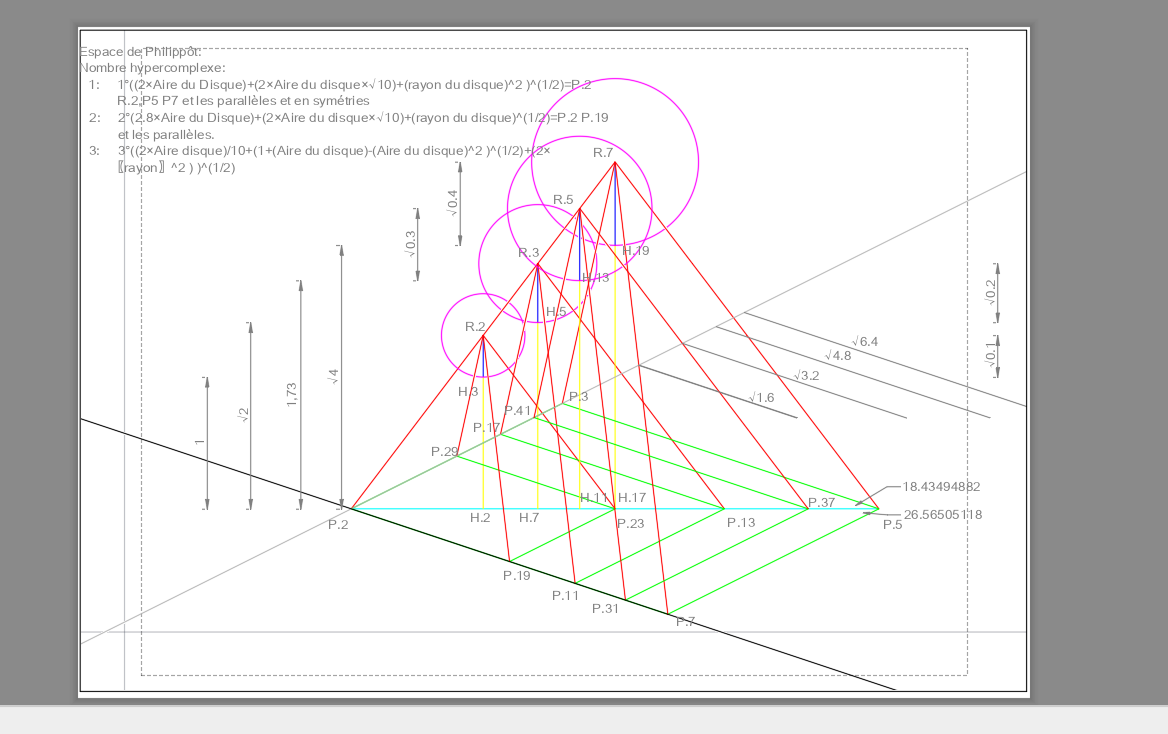
\includegraphics[width=0.95\textwidth]{espace_philippot.png}
    \caption{Illustration générale de l’Espace de Philippôt.}
\end{figure}

\section*{Introduction}

L’Espace de Philippôt constitue le cœur conceptuel du quatrième chapitre de la théorie unifiée \emph{L’univers est au carré}. Cet espace géométrique, représenté par une structure pyramidale associée à une série de disques, est construit selon la progression de la spirale de Théodore de Cyrène. Cette spirale, définie par les longueurs successives $\sqrt{1}, \sqrt{2}, \sqrt{3}, \sqrt{4}, \dots$, sert ici de base métrique pour organiser les hauteurs, les rayons et les aires qui structurent l’espace.

L’illustration ci-dessus montre la correspondance entre :
\begin{itemize}
    \item les disques supérieurs, dont les rayons suivent la progression $\sqrt{0.1}, \sqrt{0.2}, \sqrt{0.3}, \sqrt{0.4}, \dots$ ;
    \item les hauteurs de la pyramide, alignées sur les valeurs $\sqrt{1}, \sqrt{2}, \sqrt{3}, \sqrt{4}, \dots$ ;
    \item les points géométriques notés $H.2$, $H.3$, $H.5$, $H.7$, $H.11$, $H.13$, $H.17$, $H.19$, qui marquent les niveaux successifs de la spirale.
\end{itemize}

Une convention fondamentale de cet espace est l’égalité :
\[
\pi = \sqrt{10},
\]
qui permet d’harmoniser les aires circulaires avec les volumes pyramidaux et ellipsoïdaux.

\section*{1. Structure géométrique de l’Espace de Philippôt}

La pyramide représentée dans la figure est construite de manière à ce que chaque hauteur corresponde à une valeur de la spirale de Théodore. Les disques situés au sommet possèdent des rayons proportionnels à ces hauteurs, selon la relation :
\[
r_n = \sqrt{0.1\,n}.
\]

Ainsi, la géométrie de l’espace est entièrement déterminée par la progression racinaire, ce qui confère à l’ensemble une cohérence interne remarquable.

\section*{2. Nombres hypercomplexes géométriques}

Les nombres hypercomplexes définis dans cet espace ne sont pas les quaternions classiques, mais une construction géométrique analogue fondée sur trois composantes :
\[
H = \left( A,\, A\sqrt{10},\, r^2 \right)^{1/2},
\]
où :
\begin{itemize}
    \item $A$ est l’aire d’un disque,
    \item $A\sqrt{10}$ représente l’aire pondérée selon la convention $\pi=\sqrt{10}$,
    \item $r^2$ est le carré du rayon du disque.
\end{itemize}

\subsection*{Exemple tiré de la figure}

L’un des nombres hypercomplexes représentés dans l’illustration est :
\[
1 \cdot \left( (2 \times A_{\text{disque}}) + (2 \times A_{\text{disque}} \times \sqrt{10}) + r^2 \right)^{1/2} = P.2.
\]

Ce type d’expression encode simultanément une aire, une aire pondérée et une mesure radiale, ce qui en fait un analogue géométrique des quaternions $(A^2 + B^2 + C^2 + D^2)^{1/2}$.

\section*{3. Aires des quatre faces à la hauteur $\sqrt{2}$}

À la hauteur correspondant à $\sqrt{2}$ dans la spirale, les quatre faces de la pyramide possèdent les aires suivantes :

\begin{itemize}
    \item \textbf{Face avant} :
    \[
    (2 + \sqrt{0.4}) - (\sqrt{0.064} - 0.4)
    \]
    \item \textbf{Face droite} :
    \[
    1.2 + \sqrt{0.064}
    \]
    \item \textbf{Face arrière} :
    \[
    (2 + \sqrt{0.4}) - (1.2 + \sqrt{0.064})
    \]
    \item \textbf{Face gauche} :
    \[
    0.4 + \sqrt{0.064}
    \]
\end{itemize}

La somme totale des aires est :
\[
(\sqrt{2})^2 + (\sqrt{2} + 0.2)^2 + 0.6
= 6.064911064
= 4.8 + 2\,A_{\text{disque}}.
\]

\section*{4. Volume de la pyramide et correspondance ellipsoïdale}

Le volume de la pyramide à la hauteur $\sqrt{2}$ est donné par :
\[
V_{\text{pyramide}} = \frac{1.6 \left( \sqrt{2} + \sqrt{0.2} \right)}{3}
= 0.9927611508.
\]

Ce volume est égal à un dixième du volume d’un ellipsoïde construit selon les paramètres de l’Espace de Philippôt :
\[
\frac{1}{10} V_{\text{ellipsoïde}}
= \frac{4\sqrt{10}\,\left( \sqrt{2}(\sqrt{2}+\sqrt{0.2})\sqrt{0.8} \right)}{10}
= 0.9927611509.
\]

Ainsi, dans cet espace, la pyramide peut être interprétée comme une \emph{décomposition plane} d’un ellipsoïde volumétriquement équivalent.

\section*{5. Relations exactes validées dans HOL}

Le fichier \texttt{espace\_philippot.thy} formalise maintenant trois lois métriques
simples qui condensent la géométrie du chapitre :
\[
\bigl(\mathrm{cote}(L_{\mathrm{ref}},n)\bigr)^2 = n\,L_{\mathrm{ref}}^2,
\qquad
\bigl(\mathrm{hauteur}(n)\bigr)^2 = n,
\qquad
\bigl(\mathrm{rayon}(n)\bigr)^2 = \frac{\sqrt{n}}{10}.
\]

Ces identités montrent que la structure est pilotée par des carrés exacts :
le carré d’un côté croît linéairement avec l’indice $n$, la hauteur suit la
spirale de Théodore, et le rayon est obtenu par une seconde racine appliquée
à cette hauteur.

\begin{center}
\begin{tabular}{|c|c|c|c|}
\hline
$n$ & $\mathrm{hauteur}(n)$ & $\mathrm{rayon}(n)^2$ & $\mathrm{rayon}(n)$ \\
\hline
1 & $1$ & $0.1$ & $\sqrt{0.1} \approx 0.316227766$ \\
2 & $\sqrt{2}$ & $\dfrac{\sqrt{2}}{10}$ & $\sqrt{\dfrac{\sqrt{2}}{10}} \approx 0.376060310$ \\
3 & $\sqrt{3}$ & $\dfrac{\sqrt{3}}{10}$ & $\sqrt{\dfrac{\sqrt{3}}{10}} \approx 0.416179146$ \\
4 & $2$ & $0.2$ & $\sqrt{0.2} \approx 0.447213595$ \\
\hline
\end{tabular}
\end{center}

La table confirme numériquement ce que le script HOL établit formellement :
le passage de la hauteur au rayon n’est pas une simple analogie graphique,
mais une loi exacte sur laquelle repose la métrique de l’Espace de Philippôt.

\section*{Conclusion}

L’Espace de Philippôt unifie la spirale de Théodore, les disques racinaires, les nombres hypercomplexes géométriques et les volumes pyramidaux et ellipsoïdaux dans une structure cohérente. Cette construction constitue un pivot essentiel de la théorie \emph{L’univers est au carré}, en révélant des correspondances profondes entre géométrie discrète, surfaces circulaires et volumes continus.

\end{document}
